\documentclass{article}

% Symbols
\usepackage{recycle}
\usepackage{amsfonts, amsthm}
\usepackage{upgreek}
\usepackage{physics}
\usepackage{cancel}
\usepackage{amssymb, latexsym, amsmath}

% Proof
\renewcommand*{\proofname}{\textbf{Demostraci\'on:}}

% Graphics
\usepackage{graphicx}
\usepackage{pgf}

% Color a letras.
%\usepackage[usenames,dvipsnames,svgnames,table]{xcolor} 

% Tikz
\usepackage{tikz}
\usetikzlibrary{arrows,automata}
\usepackage{tikz}
\usetikzlibrary{arrows,automata}

\usetikzlibrary{shapes,calc}
\tikzstyle{edge}=[shorten <=2pt, shorten >=2pt,
  >=stealth, line width=1.1pt]
\tikzstyle{blueE}=[shorten <=2pt, shorten >=2pt,
  >=stealth, line width=1.5pt, blue]
\tikzstyle{blackV}=[circle, fill=black,
  minimum size=6pt,
  inner sep=0pt, outer sep=0pt]
\tikzstyle{blueV}=[circle, fill=blue, draw,
  minimum size=6pt, line width=0.75pt,
  inner sep=0pt, outer sep=0pt]
\tikzstyle{redV}=[circle, fill=red, draw,
  minimum size=6pt, line width=0.75pt,
  inner sep=0pt, outer sep=0pt]
\tikzstyle{redSV}=[semicircle, fill=red, minimum
  size=3pt, inner sep=0pt, outer sep=0pt,
  rotate=225]
\tikzstyle{blueSV}=[semicircle, fill=blue, minimum
  size=3pt, inner sep=0pt, outer sep=0pt,
  rotate=225]
\tikzstyle{blackSV}=[semicircle, fill=black, minimum
  size=3pt, inner sep=0pt, outer sep=0pt,
  rotate=225]
\tikzstyle{vertex}=[circle, draw, minimum size=6pt,
  line width=0.75pt, inner sep=0pt,
  outer sep=0pt]

% Margins
\addtolength{\voffset}{-1cm}
\addtolength{\hoffset}{-1.5cm}
\addtolength{\textwidth}{3cm}
\addtolength{\textheight}{2cm}

%Header-Footer
\usepackage{fancyhdr}
\renewcommand{\headrulewidth}{1pt}

\newcommand{\set}[1]{%
  \left\{ #1 \right\}%
}

\pagenumbering{gobble}
\footskip = 50pt
\renewcommand{\headrulewidth}{1pt}

\pagestyle{fancyplain}

\begin{document}
\title{UNIVERSIDAD AUTÓNOMA DE MÉXICO\\ Facultad de Ciencias}
\author{Autores:  Fernanda Villafán Flores
  \\ Fernando Alvarado Palacios
  \\ Adrián Aguilera Moreno}
\date{}
\maketitle
\begin{center}
  
\includegraphics[scale=0.20]{../Imagen/Portada.jpg}\\[0.4cm]
  \Large
  \bf{Gráficas y Juegos}
  \normalsize
\end{center}
\newpage
\fancyhead[r]{ Gr\'aficas y Juegos 2021-2 }
\section*{\LARGE{Tarea 1}}

\begin{enumerate}
  %%%%%%%%%%%%%%%%%%%%%%%%%%%%%%%%% 1 %%%%%%%%%%%%%%%%%%%%%%%%%%%%%%%%%%%%%%%%%%%
\item Sea $n$ un entero, $n \ge 3$.   Demuestre que existe un \'unico
  $n$-ciclo, salvo isomorfismo.
  %%%%%%%%%%%%%%%%%%%%%%%%%%%%%%%%% 2 %%%%%%%%%%%%%%%%%%%%%%%%%%%%%%%%%%%%%%%%%%%
\item De un ejemplo de tres gr\'aficas del mismo orden, mismo tama\~no y misma
  sucesi\'on de grados tales que cualesquiera dos de dichas gr\'aficas no sean
  isomorfas, al menos una de ellas sea conexa, y al menos una sea inconexa.
  
  A continuación se muestran las gráficas: $G_1, G_2$ y $G_3$:
  
  \begin{figure}[ht!]
    \centering
    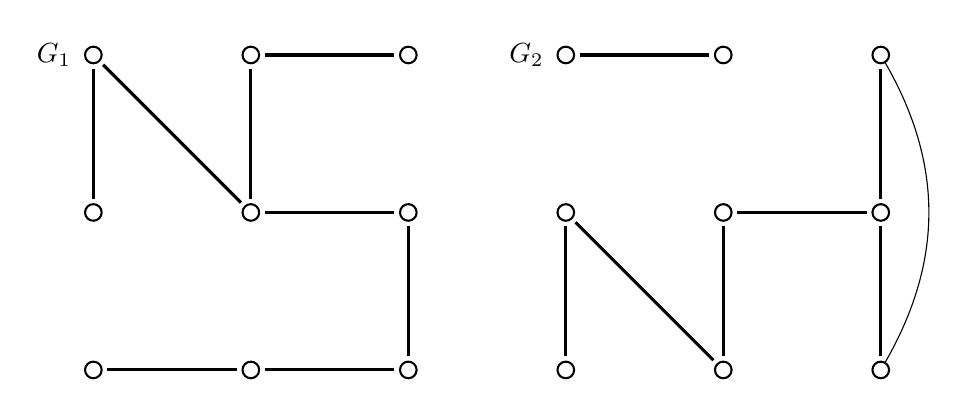
\begin{tikzpicture}
      %%%%%  Componente izquierda  %%%%%
      \node (0) [vertex,label=180:] at (0,1){};
      \node (1) [vertex,label=90:]  at (2,1){};
      \node (2) [vertex,label=90:]  at (4,1){};
      \node (3) [vertex,label=90:]  at (0,-1){};
      \node (4) [vertex,label=90:]  at (2,-1){};
      \node (5) [vertex,label=90:]  at (4,-1){};
      \node (6) [vertex,label=90:]  at (0,-3){};
      \node (7) [vertex,label=90:]  at (2,-3){};
      \node (8) [vertex,label=90:]  at (4,-3){};

      \draw [edge] (0) to (3);
      \draw [edge] (0) to (4);
      \draw [edge] (1) to (4);
      \draw [edge] (1) to (2);
      \draw [edge] (4) to (5);
      \draw [edge] (5) to (8);
      \draw [edge] (6) to (7);
      \draw [edge] (7) to (8);

      \node (L) at (-0.5,1){$G_1$};

      %%%%% Componente derecha  %%%%%
      \begin{scope}[xshift=6cm]
        \node (9) [vertex,label=180:] at (0,1){};
        \node (10) [vertex,label=90:]  at (2,1){};
        \node (11) [vertex,label=90:]  at (4,1){};
        \node (12) [vertex,label=90:]  at (0,-1){};
        \node (13) [vertex,label=90:]  at (2,-1){};
        \node (14) [vertex,label=90:]  at (4,-1){};
        \node (15) [vertex,label=90:]  at (0,-3){};
        \node (16) [vertex,label=90:]  at (2,-3){};
        \node (17) [vertex,label=90:]  at (4,-3){};

        \draw [edge] (9)  to (10);
        \draw [edge] (11) to (14);
        \draw [edge] (12) to (16);
        \draw [edge] (12) to (15);
        \draw [edge] (13) to (14);
        \draw [edge] (13) to (16);
        \draw [edge] (14) to (17);
        \path(11)edge[bend left]node{}(17);
        \node (L) at (-0.5,1){$G_2$};
      \end{scope}
    \end{tikzpicture}
  \end{figure}

  \begin{figure}[ht!]
    \centering
    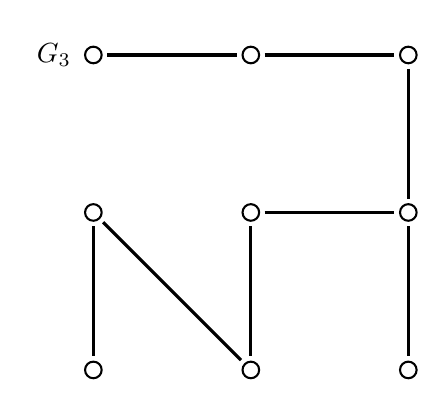
\begin{tikzpicture}
      %%%%% Componente debajo  %%%%%
      \node (0) [vertex,label=180:] at (0,1){};
      \node (1) [vertex,label=90:]  at (2,1){};
      \node (2) [vertex,label=90:]  at (4,1){};
      \node (3) [vertex,label=90:]  at (0,-1){};
      \node (4) [vertex,label=90:]  at (2,-1){};
      \node (5) [vertex,label=90:]  at (4,-1){};
      \node (6) [vertex,label=90:]  at (0,-3){};
      \node (7) [vertex,label=90:]  at (2,-3){};
      \node (8) [vertex,label=90:]  at (4,-3){};

      \draw [edge] (0) to (1);
      \draw [edge] (1) to (2);
      \draw [edge] (2) to (5);
      \draw [edge] (3) to (6);
      \draw [edge] (3) to (7);
      \draw [edge] (4) to (5);
      \draw [edge] (4) to (7);
      \draw [edge] (5) to (8);

      \node (L) at (-0.5,1){$G_3$};
    \end{tikzpicture}
  \end{figure}
  
  con sucesiones orden $9$, tamaño $8$ y sucesión de grados $(1,1,1,2,2,2,2,2,3)$.
  \hfill $\square$
%%%%%%%%%%%%%%%%%%%%%%%%%%%%%%%%% 3 %%%%%%%%%%%%%%%%%%%%%%%%%%%%%%%%%%%%%%%%%%%
\item Sea $D$ una digr\'afica.   Demuestre que
  $$\sum_{v \in V_D} d^+(v) = \sum_{v \in V_D} d^-(v) = |A_D|.$$
  
  \renewcommand\qedsymbol{QED}
  \begin{proof}
    La demostración se dividirá en dos incisos:  
    \begin{itemize}
    \item[$\cdot$)] $\displaystyle \sum_{v \in V_{D}} d^{+}(v) = \abs{A_{D}}$ 
      
      Sea $M_{1}$ una matriz de incidencia de $D$, tal que:
      \begin{center}
        $M_{1} = M^{+}_{ij}
        = \left \{ 
        \begin{array}{lcc}
          1 &   si  & v_{i} \hspace{0.3em} es \hspace{0.3em} la
          \hspace{0.3em} cola \hspace{0.3em} de \hspace{0.3em} e_{j} \\
          \\0 &  si & v_{i} \hspace{0.3em} no \hspace{0.3em} es \hspace{0.3em}
          la \hspace{0.3em} cola \hspace{0.3em} de \hspace{0.3em} e_{j}
        \end{array}
        \right.$
      \end{center}
      Ahora, supongamos que $V = \{v_{1}, \dotsm, v_{n}\}$ donde $v_{i}$
      corresponde al \textit{i-ésimo} renglón de $M_{1}$.
      
      Sabemos que las entradas de cada columna de $M_{1}$ son igual a 1,
      que son las flechas $e_{j}$ con un vértice llamado \textit{cola de la flecha}.
      Por otro lado, las entradas del \textit{i-ésimo} renglón de $M_{1}$
      suman $d^{+}(v_{i})$, ya que las entradas corresponden a todas las
      flechas de las cuales $v_{i}$ es cola de dicha flecha. 
      
      Entonces, tenemos que:
      \begin{equation*}
        \begin{split}
          \abs{A_{D}} & = \sum_{j=1}^{\abs{A}} \sum_{i=1}^{\abs{V}} M^{+}_{ij} \\
          & = \sum_{i=1}^{\abs{V}} \sum_{j=1}^{\abs{A}} M^{+}_{ij} \\
          & = \sum_{i=1}^{\abs{V}} d^{+}(v_{i}) \\
          & = \sum_{v \in V} d^{+}(v)
        \end{split}
      \end{equation*}
      De forma análoga se realiza el otro inciso.
      
    \item[$\cdot\cdot$)] $\displaystyle \sum_{v \in V_{D}} d^{-}(v) = \abs{A_{D}}$ 
      
      Sea $M_{2}$ una matriz de incidencia de $D$, tal que:
      \begin{center}
        $M_{2} = M^{-}_{ij}
        = \left \{ 
        \begin{array}{lcc}
          1 &   si  & v_{i} \hspace{0.3em} es \hspace{0.3em} la \hspace{0.3em}
          cabeza \hspace{0.3em} de \hspace{0.3em} e_{j} \\
          \\0 &  si & v_{i} \hspace{0.3em} no \hspace{0.3em} es \hspace{0.3em}
          la \hspace{0.3em} cabeza \hspace{0.3em} de \hspace{0.3em} e_{j}
        \end{array}
        \right.$
      \end{center}
      Ahora, supongamos que $V = \{v_{1}, \cdots, v_{n}\}$ donde $v_{i}$
      corresponde al \textit{i-ésimo} renglón de $M_{1}$.
      
      Sabemos que las entradas de cada columna de $M_{1}$ son igual a 1,
      que son las flechas $e_{j}$ con un vértice llamado \textit{cabeza de la flecha}.
      Por otro lado, las entradas del \textit{i-ésimo} renglón de $M_{1}$
      suman $d^{-}(v_{i})$, ya que las entradas corresponden a todas las
      flechas de las cuales $v_{i}$ es cabeza de dicha flecha. 
      
      Entonces, tenemos que:
      \begin{equation*}
        \begin{split}
          \abs{A_{D}} & = \sum_{j=1}^{\abs{A}} \sum_{i=1}^{\abs{V}} M^{-}_{ij} \\
          & = \sum_{i=1}^{\abs{V}} \sum_{j=1}^{\abs{A}} M^{-}_{ij} \\
          & = \sum_{i=1}^{\abs{V}} d^{-}(v_{i}) \\
          & = \sum_{v \in V} d^{-}(v)
        \end{split}
      \end{equation*}
    \end{itemize}
    Por lo tanto, queda demostrado que:
    \[
    \displaystyle \sum_{v \in V_D} d^+(v) = \sum_{v \in V_D} d^-(v) = |A_D|
    \]
  \end{proof}

  %%%%%%%%%%%%%%%%%%%%%%%%%%%%%%%%% 4 %%%%%%%%%%%%%%%%%%%%%%%%%%%%%%%%%%%%%%%%%%%
\item  Sea $n$ un entero positivo. Definimos a la {\em Ret\'icula Booleana},
  $BL_n$, como la gr\'afica cuyo conjunto de vértices es el conjunto de todos
  los posibles subconjuntos de $\set{1, \cdots, n}$, donde dos subconjuntos
  $X$ y $Y$ son adyacentes si y s\'olo si su diferencia sim\'etrica tiene
  exactamente un elemento.
  
  \begin{enumerate}
  \item Dibuje $BL_1, BL_2, BL_3$ y $BL_4$.
    
    %-------------------------- inciso (a) ---------------------
    %~~~~~~~~~~~~~~~~~~~~~~~~~~~~~~~~~~~~~~~~~~ BL_1
    Gráfica representativa de $BL_1$:
    \begin{center}
      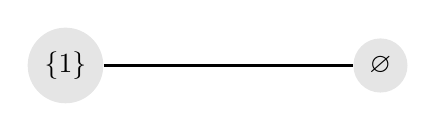
\begin{tikzpicture}
        \tikzstyle{vertex} = [circle, fill = black!10]
        \tikzstyle{edge}   = [-, thick]
        
        \node[vertex](v1)  at (0,0)  {$\{1\}$};
        \node[vertex](v2)  at (4,0)  {$\varnothing$};
        %%------------ Aristas ---------
        \draw[edge](v1)--(v2);
      \end{tikzpicture}
    \end{center}
    
    %~~~~~~~~~~~~~~~~~~~~~~~~~~~~~~~~~~~~~~~~~~ BL_2
    Gráfica representativa de $BL_2$:
    \begin{center}
      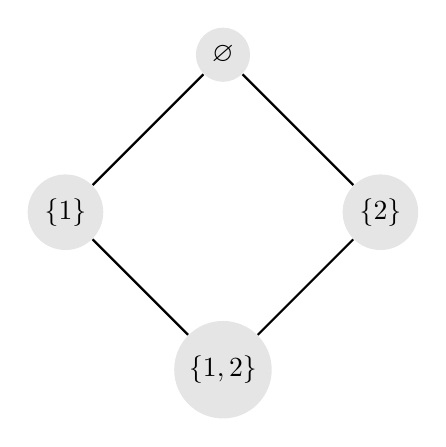
\begin{tikzpicture}
        \tikzstyle{vertex} = [circle, fill = black!10]
        \tikzstyle{edge}   = [-, thick]
        
        \node[vertex](v1)  at (0,2)  {$\{1\}$};
        \node[vertex](v2)  at (4,2)  {$\{2\}$};
        \node[vertex](v3)  at (2,0)  {$\{1,2\}$};
        \node[vertex](v4)  at (2,4)  {$\varnothing$};
        
        %%------------ Aristas ---------
        \draw[edge](v1)--(v3);
        \draw[edge](v1)--(v4); 
        \draw[edge](v2)--(v3);
        \draw[edge](v2)--(v4);
      \end{tikzpicture}
    \end{center}
    
    %~~~~~~~~~~~~~~~~~~~~~~~~~~~~~~~~~~~~~~~~~~~ BL_3
    Gráfica representativa de $BL_3$:
    \begin{center}
      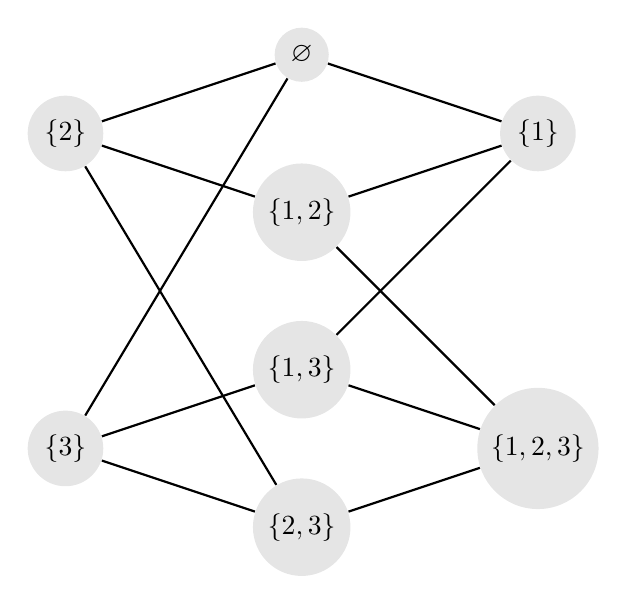
\begin{tikzpicture}
        \tikzstyle{vertex} = [circle, fill = black!10]
        \tikzstyle{edge}   = [-, thick]
        
        \node[vertex](v1)  at (0,1)  {$\{3\}$};
        \node[vertex](v2)  at (0,5)  {$\{2\}$};
        \node[vertex](v3)  at (3,0)  {$\{2,3\}$};
        \node[vertex](v4)  at (3,2)  {$\{1,3\}$};
        \node[vertex](v5)  at (3,4)  {$\{1,2\}$};
        \node[vertex](v6)  at (3,6)  {$\varnothing$};
        \node[vertex](v7)  at (6,1)  {$\{1,2,3\}$};
        \node[vertex](v8)  at (6,5)  {$\{1\}$};
        
        %%------------ Aristas ---------
        \draw[edge](v1)--(v3);
        \draw[edge](v1)--(v4);
        \draw[edge](v1)--(v6);
        \draw[edge](v2)--(v3);
        \draw[edge](v2)--(v5);
        \draw[edge](v2)--(v6);
        \draw[edge](v8)--(v4);
        \draw[edge](v8)--(v5);
        \draw[edge](v8)--(v6);
        \draw[edge](v7)--(v3);
        \draw[edge](v7)--(v4);
        \draw[edge](v7)--(v5);
      \end{tikzpicture}
    \end{center}
    
    %~~~~~~~~~~~~~~~~~~~~~~~~~~~~~~~~~~~~~~~~~~~ BL_4
    Gráfica representativa de $BL_4$:
    \begin{center}
      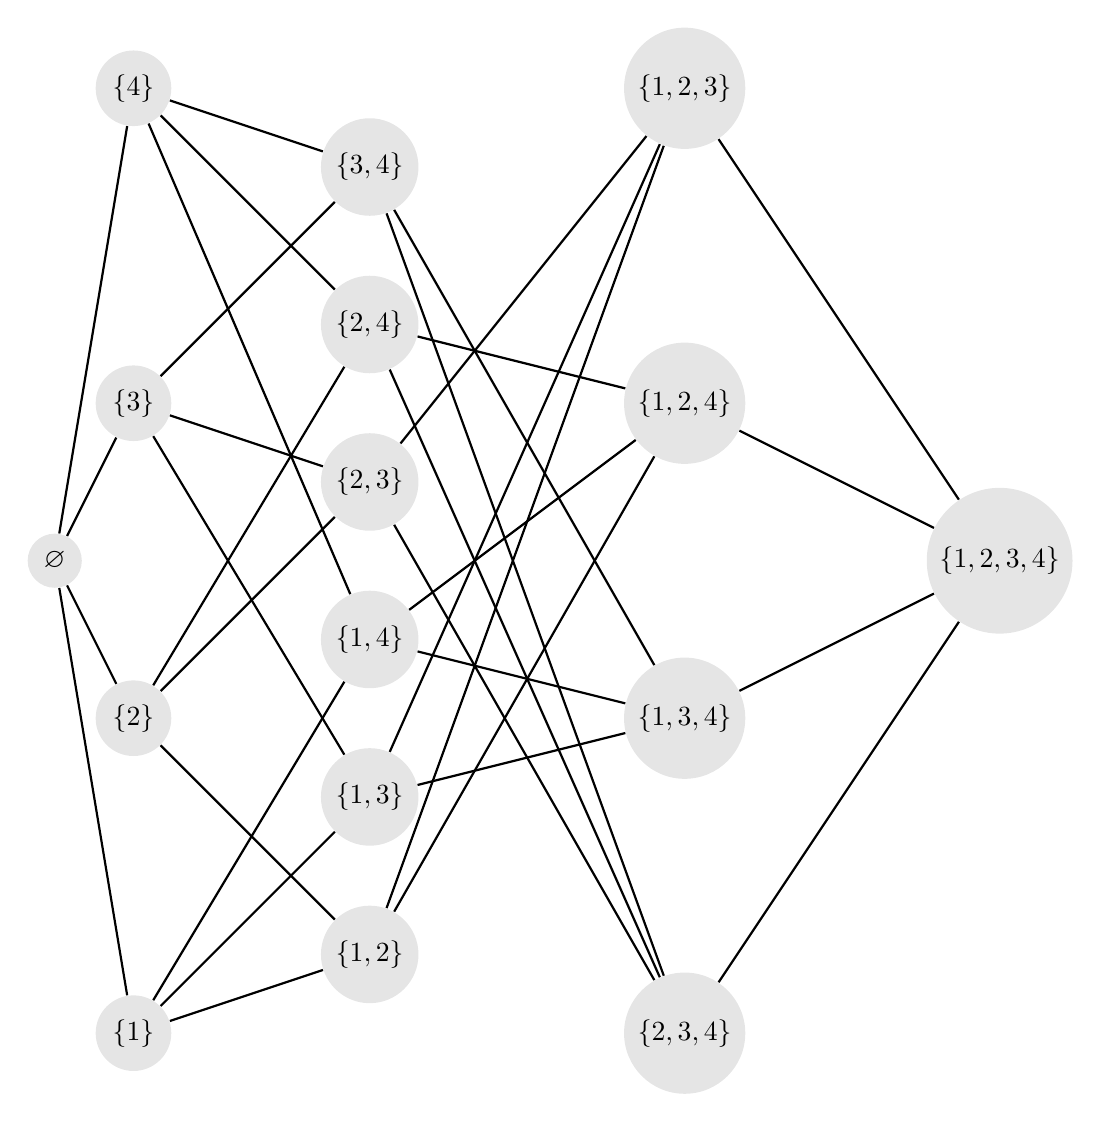
\begin{tikzpicture}
        \tikzstyle{vertex} = [circle, fill = black!10]
        \tikzstyle{edge}   = [-, thick]
        
        \node[vertex](v1)   at (0,6)    {$\varnothing$};
        \node[vertex](v2)   at (1,0)    {$\{1\}$};
        \node[vertex](v3)   at (1,4)    {$\{2\}$};
        \node[vertex](v4)   at (1,8)    {$\{3\}$};
        \node[vertex](v5)   at (1,12)   {$\{4\}$};
        \node[vertex](v6)   at (4,1)    {$\{1,2\}$};
        \node[vertex](v7)   at (4,3)    {$\{1,3\}$};
        \node[vertex](v8)   at (4,5)    {$\{1,4\}$};
        \node[vertex](v9)   at (4,7)    {$\{2,3\}$};
        \node[vertex](v10)  at (4,9)    {$\{2,4\}$};
        \node[vertex](v11)  at (4,11)   {$\{3,4\}$};
        \node[vertex](v12)  at (8,12)   {$\{1,2,3\}$};
        \node[vertex](v13)  at (8,8)    {$\{1,2,4\}$};
        \node[vertex](v14)  at (8,4)    {$\{1,3,4\}$};
        \node[vertex](v15)  at (8,0)    {$\{2,3,4\}$};
        \node[vertex](v16)  at (12,6)   {$\{1,2,3,4\}$};
        
        %%------------ Aristas ---------
        \draw[edge](v1)--(v2);
        \draw[edge](v1)--(v3);
        \draw[edge](v1)--(v4);
        \draw[edge](v1)--(v5);
        \draw[edge](v2)--(v6);
        \draw[edge](v2)--(v7);
        \draw[edge](v2)--(v8);
        \draw[edge](v3)--(v6);
        \draw[edge](v4)--(v9);
        \draw[edge](v3)--(v9);
        \draw[edge](v4)--(v7);
        \draw[edge](v5)--(v8); 
        \draw[edge](v3)--(v10);
        \draw[edge](v4)--(v11);
        \draw[edge](v5)--(v11);
        \draw[edge](v5)--(v10);
        \draw[edge](v12)--(v6);
        \draw[edge](v12)--(v7);
        \draw[edge](v12)--(v9);
        \draw[edge](v13)--(v6);
        \draw[edge](v13)--(v8);
        \draw[edge](v14)--(v7);
        \draw[edge](v14)--(v8);
        \draw[edge](v15)--(v9);
        \draw[edge](v14)--(v11);
        \draw[edge](v13)--(v10);
        \draw[edge](v15)--(v11);
        \draw[edge](v15)--(v10);
        \draw[edge](v16)--(v12);
        \draw[edge](v16)--(v13);
        \draw[edge](v16)--(v14);
        \draw[edge](v16)--(v15);
      \end{tikzpicture}
    \end{center}
    \hfill $\square$

    %-------------------------- inciso (b) ---------------------
  \item Determine $|V_{BL_n}|$ y $|E_{BL_n}|$. (Justifique su respuesta).
    
    Veamos que la cantidad de vértices es igual a la
    cantidad de subconjuntos que se pueden formar de
    la retícula $BL_n$, esto es el conjunto potencia
    de $\{1, \dotsm, n\}$. Por lo que:
    \begin{center}
      $\abs{V_{BL_n}} = \abs{P \left(\{1, \dotsm, n\}\right)} = 2^{n}$
    \end{center}
    Mientras que es un tanto más empírica la forma en
    la que se obtiene la cardinalidad de $E_{BL_n}$,
    veamos la siguiente tabla con las primeras retículas:
    \begin{center}
      \begin{tabular}{|c|c|}
        \hline
        Valor de $n$ & $\#$ de aristas \\
        \hline
        $n = 1 \Rightarrow$ & $1$ arista \\
        \hline
        $n = 2 \Rightarrow$ & $4$ arista \\
        \hline
        $n = 3 \Rightarrow$ & $12$ arista \\
        \hline
        $n = 4 \Rightarrow$ & $32$ arista \\
        \hline
      \end{tabular}
    \end{center}
    Nótese que:
    \begin{eqnarray*}
      1 \cdot 1 &= 1 \cdot 2^{1-1} =& 1\\
      2 \cdot 2 &= 2 \cdot 2^{2-1} =& 4\\
      3 \cdot 4 &= 3 \cdot 2^{3-1} =& 12\\
      4 \cdot 8 &= 4 \cdot 2^{4-1} =& 32
    \end{eqnarray*}
    Podemos deducir $\abs{E_{BL_n}} = n \cdot 2^{n-1}$.
    
    \begin{center}
      \fbox{
        \begin{minipage}[b][1\height]%
          [t]{0.867\textwidth}
          En general las retículas booleanas son $n$-regulares,
          pues para un $x \in V_{BL_{n - 1}}$ con $BL_{n - 1}$
          siendo $n$-regular, el  $BL_n$ tendrá a $x$ relacionado
          con al menos $n -1$ elementos (son con los que ya se
          relacionaba en $BL_{n - 1}$) y $x$ se relacionará con
          el conjunto de tamaño $|x| + 1$ (el cuál sólo es uno,
          pues este es $x \cup \{n\}$) y concluimos que $BL_n$
          es $n$-regular, pues cada $x$ se relaciona con
          $(n - 1) + 1$ elemento.
      \end{minipage}}
    \end{center}
    
    Luego hay $n$ aristas por cada vértice (los cuáles son
    $2^n$, como ya vimos) y por el inciso ($c$) tenemos que
    $BL_n$ es bipartita, esto aunado al hecho de que es
    $n$-regular, nos da partes en $BL_n$ de igual
    cardinalidad. De lo anterior hay una cantidad de aristas
    igual a $n$ por cada una de las partes, \textit{i.e.},
    \begin{eqnarray*}
      |E_{BL_n}| &=& n \cdot \frac{2^n}{2}\\
      &=& n \cdot 2^{n - 1}
    \end{eqnarray*}

        
    \hspace*{4 cm} $\therefore\ \ \ \ \ \abs{V_{BL_n}} = 2^n
    \text{ y } |E_{BL_n}| = n \cdot 2^{n -1}$
    \hfill $\square$
    
    %-------------------------- inciso (c) ---------------------
    
  \item Demuestre que $BL_n$ es bipartita para cualquier $n \in \mathbb{Z}^+$. 
    
    \begin{proof}
      
      Sea $A = \{1, \dotsm,n\}$ conjunto con $n \in \mathbb{Z}^+$.     
      Veamos que podemos particionar nuestra $BL_n$ en los conjuntos
      $X$ y $Y$ de tal forma que $X$ contenga los subconjuntos de
      $BL_n$ tales que su cardinalidad es $2k$, donde $2k \in A$  y
      $Y$ tal que contenga los subconjuntos de $BL_n$ de cardinalidad
      $2k -1$, donde $2k -1 \in A$.
      
      Veamos que pasa cuando dos subconjuntos en $BL_n$ se relacionan,
      es decir, son adyacentes en $BL_n$.
      \begin{itemize}
      \item[-] Su diferencia simétrica es $1$.
      \end{itemize}
      Dados dos subconjuntos en $BL_n$, uno de ellos debe tener cardinalidad
      $n+1$ o $n-1$ y el otro de cardinalidad $n$ tal que se cumple que uno
      de ellos es subconjunto del otro.
      
      Notemos que en $X$ están todos los subconjuntos de cardinalidad par.
      Por tanto, la diferencia simétrica entre cualesquiera 2 subconjuntos
      distintos en $X$ es:
      \begin{itemize}
      \item[-] A lo menos un conjunto de cardinalidad $2$.
      \end{itemize}
      De lo anterior, tenemos que ningún subconjunto en
      $X$ cumple ser adyacente mediante la definición de $BL_n$.
      
      Ahora notemos que, en $Y$ están todos los subconjuntos de
      $BL_n$  que tienen cardinalidad impar. Por lo tanto, la
      diferencia simétrica en cualesquiera dos subconjuntos
      distintos en $Y$ es:
      \begin{itemize}
      \item[-] Al menos un conjunto de cardinalidad $2$.
      \end{itemize}
      Entonces tenemos que: $2k + 1 - (2k -1) = 2$ y como $Y$
      es un conjunto, no se tiene dos conjuntos iguales a los
      cuales relacionar. Por lo anterior y por la definición de
      diferencia simétrica, no existen dos conjuntos adyacentes
      en $Y$.
      
      \hspace*{3cm}  $\therefore$ \ \ \ $BL_n$ es bipartita en $X$ y $Y$, \textit{i.e.} $BL_n[X,Y]$
    \end{proof}
  \end{enumerate}
  
  %%%%%%%%%%%%%%%%%%%%%%%%%%%%%%%%% 5 %%%%%%%%%%%%%%%%%%%%%%%%%%%%%%%%%%%%%%%%%%%
\item Sea $G[X, Y]$ una gr\'afica bipartita.
  \begin{enumerate}

    %-------------------------- inciso (a) ---------------------
  \item Demuestre que $\sum_{v \in X} d(v) = \sum_{v \in Y} d(v)$.
  \begin{proof}
    (Inducción sobre ${|Y|}$)
    
    Sea G una gráfica tal que $G[X,Y]$ y sea r cualquier Entero tal que $|X|=r$
    
    Paso base (n=1): Sea G[X,Y$_1$] donde $|X|=r$ y $|Y|=1 \Longrightarrow $ como G es bipartita, todo vértice de X se relaciona con el único elmento de Y, por lo que $\sum_{v \in X}d(v) = r $ y el grado del único vertice en Y, será igual a r, por lo tanto $\sum_{v \in X}d(v) = r = \sum_{v \in Y_1}d(v) $
    
    Hipótesis de Inducción (n=k): Supongamos que G$[X, Y_k]$ es una gráfica bipartita y que $\sum_{v \in X}d(v) = \sum_{v \in Y_k}d(v) $ 
    
    Paso inductivo (n=k+1): Sea G[X,Y$_{k+1}$] función bipartita Pd)  
    $ \sum_{v \in X} d(v) =  \sum_{v \in Y_{k+1}}d(v) $ 
    
    Demostración: Por hipotesis de inducción si  G[X,Y$_k$] $\Longrightarrow \sum_{v \in X}d(v) = \sum_{v \in Y_k}d(v) \Longrightarrow$ si agregamos un vértice a Y$_k$, donde $|Y_{k+1}|= |Y_k| +1 \Longrightarrow$ por defición de gráfica bipartica existirán vértices de X que serán adyacentes con el nuevo vértice en Y $\Longrightarrow$ sea q el número de nuevas relaciones entre X y el nuevo vértice en Y, vemos que el grado del nuevo vértice en Y será igual a q $\Longrightarrow \sum_{v \in X} d(v) = \sum_{v \in Y_k}d(v) + q =  \sum_{v \in Y_{k+1}}d(v) $ 
    
    Por lo tanto para toda g tenemos que  $\sum_{v \in X}d(v) = \sum_{v \in Y}d(v) $ 
    \end{proof}
    
    %-------------------------- inciso (b) ---------------------
  \item Demuestre que si $G$ es $k$-regular, con $k \ge 1$, entonces
    $|X| = |Y|$.
    \begin{proof}
      Dada $G$ una gráfica $k$-regular $G[X,Y]$ bipartita. 
      Sabemos que por ser bipartita y $k$-regular, se cumple que:
      \begin{itemize}
      \item[-] Al menos $|V_G|=2$, pues una gráfica tiene como mínimo
        un elemento y por ser bipartita está debe relacionarse con al
        menos un elemento en la partición ajena a ella misma. 
        
      \item[-] Todos los vértices tienen grado $k$.
      \end{itemize}
      Tenemos que en el caso mínimo, $|V_G| = 2$  hay una relación entre
      dos vértices (cada uno de ellos pertenecientes a su respectiva
      parte). Por lo tanto, al ser $k$-regular, tenemos que el grado
      de estos vértices es al menos $1$. Entonces, $k \geq 1$.
      
      Ahora usemos el resultado de $5$ ($a$). Sabemos que:
      \[
      \sum_{v \in X} d(v) = \sum_{v \in Y} d(v)
      \]
      Como cada vértice tiene grado $k$. podemos decir que:
      \[
      \abs{X} = \frac{\displaystyle \sum_{v \in X} d(v)}{k} \text{\hspace{0.3cm}
        y \hspace{0.3cm}} \abs{Y} = \frac{\displaystyle \sum_{v \in Y} d(v)}{k}
      \]
      De lo anterior, se deduce que:

      \hspace*{5.6cm} $\therefore\ \ \ \ |X| = |Y|$
    \end{proof}
  \end{enumerate}
  
\end{enumerate}

%%%%%%%%%%%%%%%%%%%%%%%%%%%%%%%% Extras %%%%%%%%%%%%%%%%%%%%%%%%%%%%%%%%%%%%%%%%
\subsection*{Puntos Extra}

\begin{enumerate}
\item Sea $G = [X, Y]$ una gr\'afica bipartita con $|X| = r$ y $|Y| = s$.
  \begin{enumerate}
  \item Demuestre que $|E| \le rs$.
%---------------------------------------------------------------------------------------------
\begin{proof}
  (Inducción sobre $|Y|$) 
  
  Sea r cualquier Entero tal que $|X|=r$
  
  Paso base $(n = 1)$: Sea G($V_1$,$E_1$): $G[X,Y]$ donde $|Y|=1\Longrightarrow$  se sigue por vacuidad que MAX$\{|E_1|\}$=r (ya que todo elemento de X solo se puede relacionar al unico vértice  en Y). 
  
  Hipótesis de inducción($ n = k$): Supongamos que existe G(V$_k$, E$_k$): G[X,Y] tal que $|X|=r$ y $|Y|= k$ $\Longrightarrow$ MAX$\{|E_k|\} = rk$
  
  Pd) (para n=k+1): G(V$_{(k+1)}$,E$_{(k+1)}$): G[X,Y] tal que $|X|=r$ y $|Y|=k+1 \Longrightarrow$ 
  MAX$\{|E_{(k+1)}|\} = r(k+1)$
  
  Dem
  
  Por Hipótesis de inducción si G(V$_k$,E$_k$): G(X,Y) tal que $|X|=r$ y $|Y|=k$ por lo que 
  el MAX$\{|Ek|\}=rk $ agregando un vertice a Y $\Longrightarrow$ definimos $|V(k+1)|$ = 1 + $|Vk|$ por lo que el MAX$\{|E(k+1)|\}$ = MAX$\{|Ek|\} + $ k (donde k son las nuevas relaciones entre el vertice que se agrego y todos los vertices de X) $\Longrightarrow$ MAX$\{|Ek|\} + $ k $= rk +r = r(k+1)$
  
  por lo tanto el MAX$\{|E(k+1)|\} = r(k+1)$.
  
  Por lo tanto, para toda G(V,E) si G[X,Y]: $|X|=r$ y $|Y|=s \Longrightarrow$ MAX$\{|E|\} =$ rs
  \end{proof}
%---------------------------------------------------------------------------------------------
  \item Deduzca que $|E| \le \frac{|V|^2}{4}$.
%-----------------------------------------------------------------------------------------------
\begin{proof}
  PD. rs $ \leqslant (|V|^2)/4$
  
  Sabemos que para toda gráfica G$=[X,Y]: |X|=r$ y $|Y|=s \Longrightarrow$ (por teo. cálculo $x^2 > 0$) sean cualesquiera r,s que pertenecen a los Enteros  $\Longrightarrow  0 \leqslant (r-s)^2  \Longrightarrow 0   \leqslant r^2 + s^2 -2rs \Longrightarrow 2rs \leqslant r^2 + s^2 \Longrightarrow 4rs \leqslant r^2 + s^2 + 2rs \Longrightarrow 4rs \leqslant (r+s)^2 \Longrightarrow rs \leqslant ((r+s)^2)/4 $ y $r+s = |X|+|Y|$ por lo que por definición de particion $|X| + |Y| = |V|  \Longrightarrow (|V|^2)/4$ por inciso $(a)$ tenemos que:  $|E|\leqslant rs \leqslant (|V|^2)/4$
   por lo tanto $ |E|\leqslant (|V|^2)/4 $ 
  
  \end{proof}
%-----------------------------------------------------------------------------------------------

  \item Describa a las gr\'aficas bipartitas que cumplen la igualdad en el
    inciso anterior. Justifique su respuesta.
%------------------------
SOLUCION

Debemos ver donde se cumple la igualdad $|E|= (|V|^2)/4$

Sea $|V|= |X| + |Y| = r+s \Longrightarrow$ por la demostración del inciso del inciso $(b)$ y $(a)$ tenemos que si $0\leqslant(r-s)^2 \Longrightarrow |E|\leqslant rs \leqslant (|V|^2)/4 \Longrightarrow$ si $0=(r-s)^2 \Longrightarrow 0=r-s \Longrightarrow s=r \Longrightarrow rs=(|V|^2)/4 $ y si G es una gráfica bipartita completa $\Longrightarrow |E|=rs=(|V|^2)/4$ por lo tanto, si las particiones de la gráfica tienen el mismo número de elementos y tambien la gráfica es bipartita completa se cumple la desigualdad $|E|= (|V|^2)/4$
\newpage
Ejemplo:
%\end{itemize}
\begin{figure}[ht!]                                                             
    \centering                                              
        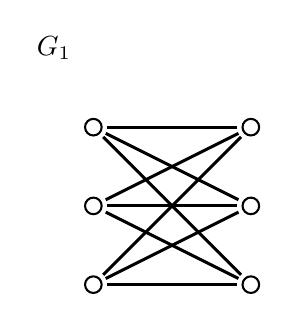
\begin{tikzpicture} 
            \node (0) [vertex,label=180:] at (0,0){};
            \node (1) [vertex,label=180:] at (0,-1){};   
            \node (2) [vertex,label=180:] at (0,-2){};   
            \node (3) [vertex,label=180:] at (2,0){};   
            \node (4) [vertex,label=180:] at (2,-1){};   
            \node (5) [vertex,label=180:] at (2,-2){};
            
         \draw [edge] (0) to (3); 
         \draw [edge] (0) to (4); 
         \draw [edge] (0) to (5); 
         \draw [edge] (1) to (3); 
         \draw [edge] (1) to (4); 
         \draw [edge] (1) to (5); 
         \draw [edge] (2) to (3); 
         \draw [edge] (2) to (4); 
         \draw [edge] (2) to (5); 
                                                                 
      \node (L) at (-0.5,1){$G_1$}; %nobre de la grafica 
    \end{tikzpicture}
\end{figure}
$rs=9$

$|E|=9$

$|V|= 9 \Longrightarrow |V|^2/4 = 36/4 = 9$
%------------------------
  \end{enumerate}

\end{enumerate}

\end{document}
